\PassOptionsToPackage{dvipsnames}{xcolor}
\documentclass{beamer}
\usepackage{xcolor}
\usepackage{pgfpages}

\usepackage[style=authortitle]{biblatex}

\setbeameroption{show notes on second screen}

\usepackage[utf8]{inputenc}
\usepackage[T1]{fontenc}
\usepackage{lmodern}
\usepackage{fontawesome}

\usepackage{minted}

\usepackage{listings}

\usepackage[american]{babel}

\usepackage{
    amsmath,
    amsfonts,
    amssymb
}

\usepackage[os=win]{menukeys}

\usetheme{UOS}

\graphicspath{{img/}}

% use this with \begin{pythoncode} ... \end{pythoncode}
\newminted{python}{linenos=false}

\newminted[outputcode]{text}{linenos=false}

% this gets rid of red boxes around syntax errors in minted
\AtBeginEnvironment{minted}{%
  \renewcommand{\fcolorbox}[4][]{#4}}

% removes the prefix "Figure 1:" in figure captions
\setbeamertemplate{caption}{\raggedright\insertcaption\par}


\begin{document}

\title[Recursion]{Week 10: Recursion}
\subtitle{Basic Programming in Python}

\date{\today}

\begin{frame}[plain]
     \titlepage
\end{frame}

\begin{frame}
    \tableofcontents
\end{frame}

\section{Fibonacci}

\begin{frame}
    \sectionpage
\end{frame}


\begin{frame}{The Fibonacci Number}

\textbf{Definition:}


$F_0 = 0, F_1 = 1$

$F_n = F_{n-1} + F_{n-2}$

\vspace{1em}
\textbf{Example:}


$F_2 = F_1 + F_0 = 0 + 1 = 1$

$F_3 = F_2 + F_1 = 1 + 1 = 2$

$F_{100} = ?$

\note{
    \begin{center}
        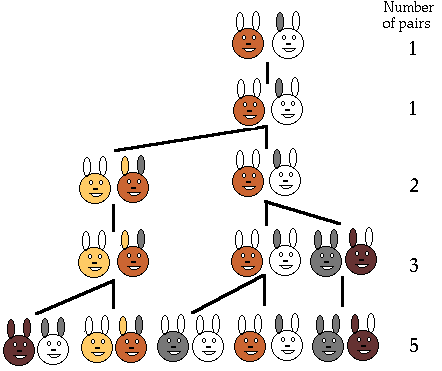
\includegraphics[height=0.8\textheight]{10_Recursion/rabbits.png}
    \end{center}

}
\end{frame}

\end{document}
